\documentclass[../main.tex]{subfiles}
\graphicspath{{\subfix{../images/}}}
\begin{document}
    \section{Formelzeichen- und Abkürzungsverzeichnis}
    \begin{tabular}{lll}
        Formelzeichen & Einheit & Beschreibung
        \\
        \hline 
        $F$ & $N$ & Kraft
        
    \end{tabular}
    \newpage
    \lipsum[1-2]
    Wir führen im volgenden das formelzeichen \gls{Spannung} 
    
    eine leerzeile macht ein kleinen absatz\\
    wenn du nur ein doppelbackslash nimmst ist es ein reiner Zeilenumbruch ohne absatz\\
    
    Wenn du aber jetzt doppelbackslash mit einer Leerzeile verbindest bekommst du einen echten Absatz.
    Desweiteren haben wir hier ein bild einbebunden, sichtbar als Grafik Abb.~\ref{fig:einBild}
    
    \begin{figure}[H]
    	\centering
    	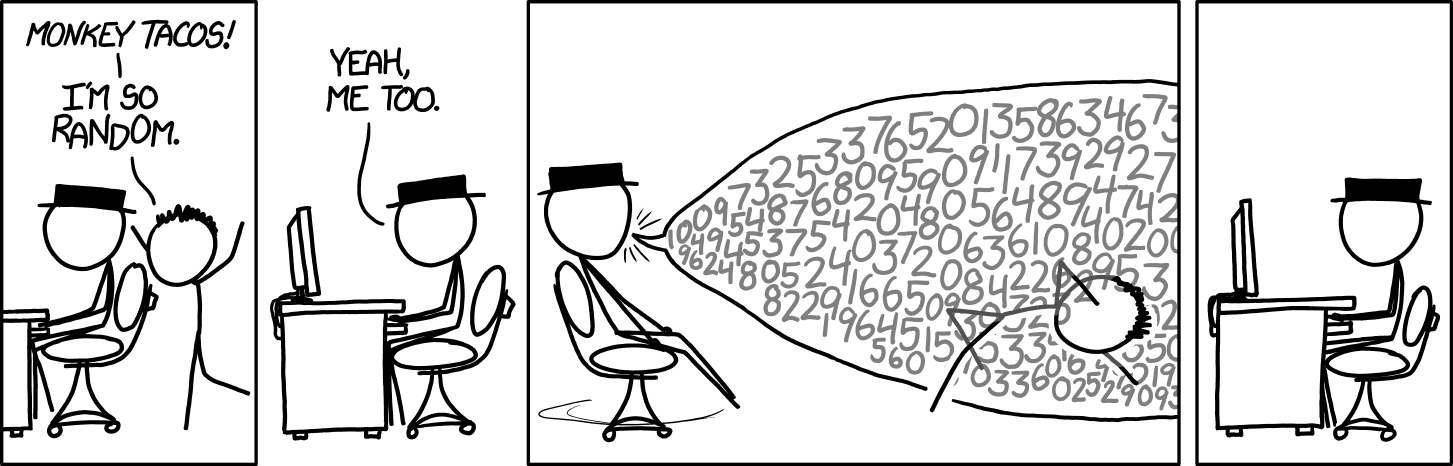
\includegraphics[width=0.5\textwidth]{im_so_random_2x.png}
    	\caption[nur kurz fürs verzeichnis]{Dies ist eine Bildunterschrift. Das kann auch ein sehr langer text werden weil wir hier viele worte mit wurstfingern tippen}
    	\label{fig:einBild}
    \end{figure}
    potatoe
    für tabellen Tab.~\ref{tab:blabla}:
    
    \begin{table}[H]
    	\caption[kurz]{bei tabellen oberhalb}
    	\label{tab:blabla}
    	\centering
    	\begin{tabular}{|l|c|r|}
    		\hline
    		linksbündig & zentriert& rechtsbündig\\
    		\hline
    		l & c&r\\
    		\hline\hline
    	\end{tabular}
    \end{table}
    
\end{document}